\documentclass[10pt,twocolumn,letterpaper, english]{article}
%
\usepackage{cvpr}
\usepackage{times}
\usepackage{epsfig}
\usepackage{graphicx}
\usepackage{lipsum}
\usepackage{multicol}
\usepackage{amsmath}
\usepackage{amssymb}
\usepackage{amsthm}
\usepackage{algorithm,algcompatible,algpseudocode}
\usepackage{multirow}

\algnewcommand\INPUT{\item[\textbf{Input:}]}%
\algnewcommand\OUTPUT{\item[\textbf{Output:}]}%



% Include other packages here, before hyperref.

% If you comment hyperref and then uncomment it, you should delete
% egpaper.aux before re-running latex.  (Or just hit 'q' on the first latex
% run, let it finish, and you should be clear).
\usepackage[breaklinks=true,bookmarks=false]{hyperref}

\cvprfinalcopy % *** Uncomment this line for the final submission

\def\cvprPaperID{****} % *** Enter the CVPR Paper ID here
\def\httilde{\mbox{\tt\raisebox{-.5ex}{\symbol{126}}}}

% Pages are numbered in submission mode, and unnumbered in camera-ready
%\ifcvprfinal\pagestyle{empty}\fi

\newcommand{\sign}{\mathop{\mathrm{sign}}}
\newcommand{\argmin}{\mathop{\mathrm{argmin}}}
\newcommand{\argmax}{\mathop{\mathrm{argmax}}}
%cose per gli enunciati
\theoremstyle{definition}
\newtheorem{definizione}{Definizione}[section]
%
\theoremstyle{plain}
\newtheorem{theo}{Theorem}[subsection]
%
\theoremstyle{plain}
\newtheorem{lemma}{Lemma}[subsection]
%
\theoremstyle{plain}
\newtheorem{corollario}{Corollario}[section]
%
\theoremstyle{plain}
\newtheorem{prop}{Proposition}[subsection]
%
\theoremstyle{remark}
\newtheorem{osservazione}{Observation}[section]

\theoremstyle{remark}
\newtheorem{ass}{Assumption}[subsection]
%
\theoremstyle{definition}
\newtheorem{esempio}{Esempio}[section]
%
\theoremstyle{definition}
\newtheorem{dimostrazione}{Proof}[section]

\theoremstyle{definition}
\newtheorem{problema}{Problema}[section]

\theoremstyle{definition}
\newtheorem{algoritmo}{Algoritmo}[section]

\renewcommand{\epsilon}{\varepsilon}
\renewcommand{\theta}{\vartheta}
\renewcommand{\rho}{\varrho}
\renewcommand{\phi}{\varphi}

\setcounter{page}{1}

\begin{document}




%%%%%%%%% TITLE
\title{{\large Project for the exam - Optimization for Data Science}\\Frank-Wolfe for White Box Adversarial Attacks}

\author{Eleonora Brasola\\
{\tt\small Student n° 2007717  }
% For a paper whose authors are all at the same institution,
% omit the following lines up until the closing ``}''.
% Additional authors and addresses can be added with ``\and'',
% just like the second author.
% To save space, use either the email address or home page, not both
\and
Alberto Cocco\\
{\tt\small Student n° 2020357}
\and 
Greta Farnea\\
{\tt\small Student n° 2019052}
}

\maketitle
%\thispagestyle{empty}

%%%%%%%%% ABSTRACT
%\begin{abstract}
%   The ABSTRACT is to be in fully-justified italicized text, at the top
%   of the left-hand column, below the author and affiliation
%   information. Use the word ``Abstract'' as the title, in 12-point
%   Times, boldface type, centered relative to the column, initially
%   capitalized. The abstract is to be in 10-point, single-spaced type.
%   Leave two blank lines after the Abstract, then begin the main text.
%   Abstract should be no longer than 300 words.
%\end{abstract}

%************************
% SCALETTA 
% INTRODUCTIONS 
% - Adversarial attacks 
% - Difference between targeted and untargeted attacks 
% - Constrained optimization 

% THEORETICAL EXPLANATIONS AND ALGORITHMS 
% - PGM 
% - FGSM 
% - MI-FGSM 
% - FW-white 

% COMPUTATIONAL POINT OF VIEW 
% - Test on ImageNet subsets 
% - Try with different max it, epsilon, step sizes, norms 
% - Do both un- and targeted attacks 

% COMPARISON OF 
% - Computational cost in iterations 
% - Computational cost in time
% - Success rate

% CONCLUSIONS 


%************************ 



%%%%%%%%% BODY TEXT
\section{Introduction}

Machine learning models, like neural networks, are found to be vulnerable to \textit{adversarial examples}, that are obtained by modifying examples drawn from the data distribution. 
Models tend to misclassify such examples that are slightly different from the correctly classified examples. 
The surprising thing is that this behaviour is proper of a wide variety of machine learning models: adversarial examples reveal some blind spots in the state-of-the-art training algorithms. \\

Many hypothesis have been made to explain such behaviour, a lot of which are related with complexity and depth of the neural networks. 
In Goodfellow \cite{goodfellow}, it is shown that it is sufficient to have a simple linear model in order to fool it with adversarial examples. It is interesting to notice that an adversarial example generated for one model is often misclassified by other models, moreover these models generally agree on the output by missclassifying a single sample into the same class. This can be explained as a result of ‘adversarial directions’ being highly related to the weights vectors of the model and the fact that in order to provide an adversarial example what matter the most are these directions and not the specific points in space. Moreover different models learn similar function when trained to perform the same task. We refer to this property as \textit{transferability} of the adversarial example. \\ 

In this project, our goal is to implement four different algorithms for Adversarial Attacks. 
According to Rinaldi \cite{rinaldi}, Goodfellow \cite{goodfellow}, Dong \cite{momentum} and Chen \cite{frank}, we use the \textit{Projected Gradient}, the \textit{Fast Gradient Sign}, the \textit{Momentum Iterative Fast Gradient Sign} and the \textit{Frank-Wolfe-white} methods. 

All of these algorithms belong to the constrained optimization theory, thus their aim is to minimize (or maximize) a function and to comply some restrictions on the domain of the function. 

\subsection{Constrained optimization}

The most general definition of a constrained problem is: 
\begin{align}
    \min \,&f(x) \label{min_prob} \\
    \text{subject to } &x \in C \nonumber
\end{align}

\noindent where $f: \mathbb{R}^n \to \mathbb{R}$ is a convex function and $C \subseteq \mathbb{R}$ is a convex set.

We can define the \textit{set of feasible directions} $F(\bar{x})$ of a point $\bar{x} \in C \ne \emptyset$ as: 
\begin{align}
    F(\bar{x}) = \{ d \in \mathbb{R}^n, d \ne 0:\, &\exists \, \delta > 0 \text{ s.t. } \bar{x} + \alpha\, d \in C, \\ &\forall\, \alpha \in (0, \delta) \} . \nonumber
\end{align}

\noindent We recall this proposition: 

%\textbf{Proposition. }
\begin{prop}
 Let $x^* \in C$ be local minimum for problem \ref{min_prob} with $C \subseteq \mathbb{R}^n$ convex and $f \in C^1(\mathbb{R}^n)$. Then 
\begin{equation}
    \label{ineq}
    \nabla f(x^*)^T (x - x^*) \ge 0 \quad \forall x \in C \,. 
\end{equation}

\end{prop}


We can extend this proposition with another one that gives a necessary and sufficient condition for the global minimum: 

%\textbf{Proposition. }
\begin{prop}
Let $C \subseteq \mathbb{R}^n$ be a convex set and $f \in C(\mathbb{R}^n)$ be a convex function. A point $x^* \in C$ is a \textit{global minimum} of problem \ref{min_prob} if and only if 
\begin{equation*}
    \nabla f(x^*)^T (x - x^*) \ge 0 \quad \forall x \in C \,. 
\end{equation*}
\end{prop}

All these properties are valid for a minimization constrained problem such as \ref{min_prob}. 

They can be extended also for a maximization constrained problem, defined as: 
\begin{align*}
    \max\, &f(x) \\
    \text{subject to } &x \in C \,.
\end{align*}

It is an easy derivation since $\max f(x) \equiv \min -f(x)$. \\

One final key ingredient for constrained optimization is:\\

\textbf{Weierstrass Theorem} A continuous function in $\mathbb{R}$ over a convex set always admits both global maximum and minimum.

\subsection{Adversarial attacks}
% see Boosting Adv Attacks with Momentum 1-2 

Adversarial examples are used to evaluate the robustness of machine/deep learning models before they are effectively run. 
They are generated by little translations along the gradient direction and, in this way, they add small noise to the examples that are ‘invisible’ to the human eye. 
However, giving adversarial examples as input to machine learning models fool them making their output wrong.

One important property of the adversarial examples is their transferability. 
In fact, an adversarial example created for a single model usually is adversarial also for others. 
This reveals that different machine learning models learn the same features and capture the same important characteristics of their training data distribution. \\ 

There exists a variety of algorithms to create adversarial attacks and in this work we only see few that are based on gradient directions. 
The main idea is that, given an image as input, we modify each pixel moving along the gradient direction. 
Furthermore, we need to satisfy some restrictions in order not to go too far from the original input and to obtain an image that, to the human eye, is not different from the original one. \\

In order to define the constrained problem for adversarial attacks, we recall that in this paper we consider classifier models. 

A classifier learns a function $f(x): x \in \mathcal{X} \to y \in \mathcal{Y}$, where $x$ is the input image and $y$ is the label of the prediction and $\mathcal{X}$ and $\mathcal{Y}$ are their domain sets. 

As an error measure, we define a loss function $\ell(y, y_{\text{true}}): (y,y_{\text{true}}) \in \mathcal{Y} \times \mathcal{Y} \to \mathbb{R} $, that usually, for multi-classification purpose, is known as \textit{Categorical Cross Entropy}. 
The variable $y$ is the predicted label and the variable $y_{\text{true}}$ is the ground-truth target label of the classifier's input $x$. \\  

The main purpose of the adversarial attack algorithms is to make the classifier's output as wrong as possible. 
Thus, the problem we have to optimize is defined as: 
\begin{align}
    \max \, &\ell(x) \label{adv_prob} \\
    \text{subject to } & \Vert x - x_{\text{ori}} \Vert \le \epsilon \nonumber
\end{align}
where $\ell(x)$ is the loss function of the classifier, $x_{\text{ori}}$ is the input image, $x$ is the adversarial image and the condition is given by a norm $\Vert \cdot \Vert$ and a tolerance value $\epsilon$. 
We keep in mind that this problem can be transformed into a minimization problem by taking the opposite of $\ell(x)$ as objective function. 

The notation $\ell(x)$ can be confusing, as we are supposed to have the labels $y$ and $y_{\text{true}}$ as input. 
For simplicity, we write $\ell(x)$ instead of $\ell(y(x), y_{\text{true}}(x))$, referring to the classifier's loss function for the input $x$. 

The constraint of the problem \ref{adv_prob} ensures that the modifications we are applying are small enough, according to the value of $\epsilon$. 
The most used norms are the $\Vert \cdot \Vert_1$, $\Vert \cdot \Vert_2$ and $\Vert \cdot \Vert_{\infty}$. 
In this work, we consider only the last one, that is defined as: 
\begin{equation*}
    \Vert x \Vert_\infty = \max_{1\le i \le d} \vert x_i \vert \quad \text{for } x \in \mathbb{R}^d \,.
\end{equation*}

\subsection{Untargeted and targeted attacks} 

As said before, the adversarial attacks' goal is to make the classifier's output wrong. 
We can decide whether we want to have control of the wrong output or we just care that the classifier mistakes. 
For these purposes, there are two types of adversarial methods: \textit{untargeted} ones and \textit{targeted} ones. \\ 

For the untargeted problems, we just refer to \ref{adv_prob}. 
It does not matter which is the output label of the adversarial example, as long as the classifier is wrong and the confidence of the output is high enough. 
We are satisfied only to maximize its loss function, according to the restriction on the adversarial image.\\

For the targeted algorithms, the problem is formally a little different. 
It is not sufficient to have a high loss value, we want to make the classifier predict a specific target $y_{\text{target}}$. 
So we want to maximize $\ell(y, y_{\text{true}})$ but also to minimize $\ell(y, y_{\text{target}})$. 
It has now become a min-max problem and we combine \ref{adv_prob} with the following minimization problem:
\begin{align}
    \min \,\, &\ell(y, y_{\text{target}}) \label{targ_prob} \\ 
    \text{subject to } & \Vert x - x_{\text{ori}} \Vert \le \epsilon \nonumber \,,
\end{align}
in order to define a new constrained optimization problem for targeted adversarial attacks: 
\begin{align*}
    \max \,\, & \ell(y(x), y_{\text{true}}(x)) - \ell(y(x), y_{\text{target}}(x)) \\
    \text{subject to } & \Vert x - x_{\text{ori}} \Vert \le \epsilon \,.
\end{align*}

As done in Chen \cite{frank}, we refer only to \ref{targ_prob} for simplicity.
Therefore, from now on, our aim is to find the optimal solution of the minimization problem when we are dealing with targeted attacks. 


%------------------------------------------------------------------------

\section{Theoretical background}
Adversarial studies are relatively recent, since the first study has been published in 2013. In general the definition of an attack depends on how much information about the model an adversary can access to and they can be divided into two categories: \textit{white-box attacks} and \textit{black-box attacks}.

In this project we focus on the first type of attacks where the adversary have full access to the target model, and thus can compute efficiently the gradient. The optimization-based methods proposed for this setting are several and, as stated before, we will analyze and test 4 different methods: \textit{FGSM, PGM, MI-FGSM, FW-White}.

The \textit{FGSM} method works by linearizing the network loss function and ends in just one step. \textit{PGM} and \textit{MI-FGSM} are iterative methods that achieve better results than simple \textit{FGSM} but they both generate adversarial examples near the boundary of the perturbation set. The more recent \textit{FW-white} achieve both high success rates and good adversarial examples.

\subsection{FGSM}

Differently from the other three algorithms, the \textit{Fast Gradient Sign} method is a one-step gradient-based approach. 
It is not iterative and updates only once the input value $x_{\text{ori}}$. 

This method linearizes the cost function around the input value. 
%The idea of linearity is explored in Goodfellow \cite{goodfellow}. 
It must to be applied a perturbation $\eta$ to the original point $x_{\text{ori}}$ and, in Goodfellow \cite{goodfellow}, they suggest to use: 
\begin{equation*}
    \eta = \epsilon \sign (\nabla_x \ell(x_{\text{ori}})) \,.
\end{equation*}

Since in this work we perform both untargeted and targeted attacks, we define the update rule for each of these problem. 
\begin{align*}
    &x= x_{\text{ori}} + \epsilon \sign (\nabla_x \ell(x_{\text{ori}})) \quad \text{(untargeted)} \,;\\
    &x= x_{\text{ori}} - \epsilon \sign (\nabla_x \ell(x_{\text{ori}})) \quad \text{(targeted)} \,. 
\end{align*}

It can be noticed that what changes is only the sign before the perturbation. 
This is due to the fact that: 
\begin{enumerate}
    \item the function $\ell(x_{\text{ori}})$ stays the same for the two problems; 
    \item the untargeted attack is a maximization problem, thus we have to move along the direction of the gradient in order to find the maximum. For this reason there is the $+$ sign before the perturbation; 
    \item the targeted attack is a minimization problem, thus we move in the opposite direction of the gradient in order to find the minimum. For this reason there is the $-$ sign before the perturbation. 
\end{enumerate}

The constraint of our problem, $\Vert x - x_{\text{ori}} \Vert_\infty  < \epsilon$ is certainly satisfied and it is easy to prove. 
Each element of the tensor corresponding to the input image $x_{\text{ori}}$ is increased or decreased by exactly $\epsilon$. 
This is due to the fact that the expression  $\sign (\nabla_x \ell(x_\text{ori}))$  can take values only in $\{-1, 1\}$. 

We can deduce that the adversarial images will be on the boundary of the convex set, since we always apply the largest possible perturbation. 

\subsection{PGM}

The \textit{Projected Gradient} method is iterative and gradient-based approach. 
It is based on the fact that, considering only the direction of the gradient, without imposing any constraint, we might find a new value for $x_{k+1}$ that is outside the convex set $C$: 
\begin{equation*}
    x_{k+1} = x_k - \gamma_k \, \nabla f(x_k) \text{   might be that: } x_{k+1} \notin C \,\,.
\end{equation*}

In order to overcome this issue, the \textit{PGM} method projects back the new point to the nearest point belonging to the set $C$. 
The procedure of the algorithm is shown in the table \textbf{Algorithm \ref{PGD}}. 

\begin{algorithm}
\caption{PGM}\label{PGD}
\begin{algorithmic}[1]
\For{$k=1 \dots$}
  \State Set $ \bar{x}_k = \rho_C(x_k + s_k \nabla f(x_k))$ \Comment{if untargeted attack, with $s_k > 0$}
  \State Set $ \bar{x}_k = \rho_C(x_k - s_k \nabla f(x_k))$ \Comment{if targeted $\,\,\,$attack, with $s_k > 0$}
  \State If $\bar{x}_k$ satisfies some specific condition, then STOP
  \State Set $x_{k+1} = x_k + \gamma_k (\bar{x}_k - x_k)$ \Comment{with $\gamma_k \in (0, 1]$}
    
\EndFor
\end{algorithmic}
\end{algorithm}

For consistency in this work, we consider the projection function $\rho_C(\cdot)$ based on the infinite norm $\Vert \cdot \Vert_\infty$. 
In line 2 and 3 of the algorithm \ref{PGD}, the projection $\bar{x}_k$ over $C$ is the solution of the following minimization problem: 
\begin{equation*}
    \min_{x \in C} \Vert x - (x_k \pm s_k \nabla f(x_k)) \Vert_\infty \,. 
\end{equation*}

We define the argument of the projection $\rho_C(\cdot)$ according to the type of the attack we are considering and, as done for the \textit{FGSM}, we move along or in the opposite direction of the gradient, adding or subtracting the perturbation to $x_k$. \\

The projection function $\rho_C(\cdot)$ ensures that the final output of the algorithm satisfies the constraint. 
At the end of each iteration, the new point $x_{k+1}$ is certainly in the convex set.
The line 5 can be re-written as: 
\begin{equation*}
    x_{k+1} = x_k + \gamma_k (\bar{x}_k - x_k) = \gamma_k \bar{x}_k + (1-\gamma_k) x_k \,.
\end{equation*}
Since $\gamma_k$ is contained in $(0,1]$ and both $x_k$ and $\bar{x}_k$ are contained in the convex set $C$, the above combination is convex and this ensures that $x_{k+1} \in C$. 

\subsection{MI-FGSM}

Here we present the \textit{Momentum Iterative Fast Sign} method that is a iterative version of the simple \textit{FGSM} combined with momentum. 
The momentum method is, in general, an acceleration technique for gradient based algorithms. 
It consists in memorizing the past gradient direction in order to avoid narrow valleys, poor local minima or maxima and other issues. 
Since the \textit{FGSM} ends in one step under the assumption of linearity of the decision boundary \cite{goodfellow}, it may easily be stacked into poor local areas, thus it is a good idea to combine it with the momentum method.

One additional advantage of momentum in this setting is that it gives a good trade-off between attack ability and the transferability of the adversarial example. \\

The algorithm scheme is summarized in the \textbf{Algorithm \ref{MI_FGSM}}.

\begin{algorithm}
\caption{MI-FGSM}\label{MI_FGSM}
\begin{algorithmic}[1]
\INPUT{A real example $x$, ground-truth label $y$}
\OUTPUT{An adversarial example $x^\ast$}
\Require{Size of perturbation $\epsilon$, number of iterations $T$, step size $\gamma$, decay factor $\beta$ }

\State Fix $g_0 = 0$ and $x_{0}^\ast$ %$\gamma = \epsilon / T$
\For{$t=0$ to $T-1$}
    \State Input $x_t$ and obtain the gradient $\nabla_x J(x_t, y)$

    \State Accumulate velocity \begin{equation*}
        g_{t+1} = \beta \cdot g_t + \frac{\nabla_x J(x_t, y)}{\Vert \nabla_x J(x_t, y) \Vert_1}
    \end{equation*}
    
    \State Update \begin{align*}
        x_{t+1} = x_t + \gamma \cdot \text{sign} (g_{t+1}) \quad &\text{if untargeted attack}\\ 
        x_{t+1} = x_t - \gamma \cdot \text{sign} (g_{t+1}) \quad &\text{if targeted attack}
    \end{align*}
    
\EndFor
\end{algorithmic}
\end{algorithm}

In line 1 we initialize the gradient to zero and fix the starting point.
The momentum term can be found in line 4 with a decay factor $\beta$ and the current gradient is normalized with its $L_1$ norm in order to correct the gradients scale.
As done in the previous methods, in line 5 we choose the update rule according to the type of attack we are considering.
An adversarial example $x_{t}^{\ast}$ is perturbed in the direction of $g_t$ (or its opposite) with a step size of $\gamma$. 


\begin{osservazione}
If $\beta = 0$, the \textit{MI-FGSM} reduces to the iterative version of \textit{FGSM}, defined as \textit{I-FGSM} in literature.
\end{osservazione}


\subsection{FW-white}

The \textit{Frank Wolfe} method is an iterative first-order optimization algorithm. 
It is widely used in data science since it is a projection-free algorithm and has a smaller cost per iteration with respect to projection methods.

In this section, we present the Frank Wolfe method for \textit{white-box} attacks proposed in Chen \cite{frank}. 
The general idea of this method is to call a \textit{Linear Minimization Oracle} (LMO). 
Starting from a feasible solution, at each iteration we define a descent direction as the solution of:
\begin{equation*}
    \min_{x \in C}\nabla f(x_k)^T (x-x_k)\,.
\end{equation*}

The previous is equivalent to the linear approximation of $f(\cdot)$ in $x_k$:
\begin{equation*}
    \min_{x \in C} f(x_k) + \nabla f(x_k)^T (x-x_k)\,.
\end{equation*}

By the Weierstrass theorem, we have that a solution of such problem exists.
In the context of \textit{white-box attacks} the algorithms introduce an additional momentum $\textbf{m}_t$ term. 
The scheme is summarized in the \textbf{Algorithm \ref{FW}}.

\begin{algorithm}
\caption{FW-White}\label{FW}
\begin{algorithmic}[1]
\INPUT{Number of iterations T, step size $ \gamma$}
\OUTPUT{An adversarial example $x_T$}

\State Set $x_0 = x_{\text{ori}}$, $m_{-1} = - \nabla_x f(x_0)$ if untargeted attack, $m_{-1} = \nabla_x f(x_0)$ if targeted attack
\For{$t=0$ to $T-1$}
    \State $m_t = \beta \cdot m_{t-1} - (1-\beta) \cdot \nabla f(x_t) $ \Comment{if untargeted}
    \State $m_t = \beta \cdot m_{t-1} + (1-\beta) \cdot \nabla f(x_t) $ \Comment{if targeted}
    \State $v_t = \text{argmin}_{x \in C} \langle x, m_t \rangle = - \epsilon \cdot \sign (m_t) + x_{\text{ori}} $
    \State $d_t = v_t - x_t $
    \State $x_{t+1} = x_t + \gamma d_t $
    
\EndFor
\end{algorithmic}
\end{algorithm}

The difference between untargeted and targeted attacks in this case is a little different from the previous methods we have presented. 
This is because we want not to modify the closed-form solution of the LMO, defined in line 5. 
For this reason, instead of using two different update rules, we define the momentum term $m_t$ in different ways. 

In line 4, we propose what is done in Chen \cite{frank}; in line 3, since we have to move along the opposite direction of the movement for targeted attacks, we consider $- \nabla f(x_t)$ as the gradient of the cost function. \\

Thanks to the momentum term $m_t$, the LMO direction is stabilized and the convergence of the algorithm is found to be empirically accelerated. 

In line 5, we exploit the closed-form solution for the LMO for the $L_\infty$ norm case. 
The proof of this formulation is in the following section \ref{LMO} and here we just write the full update rule of line 7:
\begin{equation*}
    x_{t+1} = x_t - \gamma \, \epsilon \cdot \sign(m_t) - \gamma (x_t - x_{\text{ori}}) \,.
\end{equation*}
The last term of the equation above enforces $x_t$ to be close to $x_{\text{ori}}$ for all of the iterations. 
We can suppose that the final adversarial image will have smaller distortion with respect to the other algorithms and this is the main advantage of the \textit{FW} method with momentum. 

\subsubsection{LMO closed-form solution} \label{LMO}

\begin{prop}The LMO defined in line 4 has a closed-form solution both for $L_2$ and $L_\infty$. \\
\end{prop}
\begin{proof}
Let $\textbf{h}=(x - x_{\text{ori}})/ \epsilon$. Then considering line 4 we have:
\begin{align*}
    \argmin_{\Vert x - x_{\text{ori}} \Vert_p \le \epsilon} \langle x, m_t \rangle &= \argmin_{\Vert h \Vert_p \le 1} \epsilon \cdot \langle h,m_t \rangle \\
    &= \argmax_{\Vert h \Vert_p \le 1} \epsilon \cdot \langle h, -m_t \rangle 
\end{align*}

By H\"{o}lder's inequality (element wise), the maximum value is reached when: 
\begin{equation*}
    \left | h_i \right | = c \cdot \left | (m_t)_i \right |^{\frac{1}{p-1}}
\end{equation*}

Since $\Vert h \Vert_p \le 1$ we have:

\begin{equation*}
    h_i= - \frac{\sign((m_t)_i)\cdot \left | (m_t)_i \right |^{\frac{1}{p-1}}}{(\sum_{i=1}^d \left | (m_t)_i \right |^{\frac{1}{p-1}} )^{\frac{1}{p}}}
\end{equation*}

And,
\begin{equation*}
      x_i=\epsilon \cdot - \frac{\sign((m_t)_i)\cdot \left | (m_t)_i \right |^{\frac{1}{p-1}}}{(\sum_{i=1}^d \left | (m_t)_i \right |^{\frac{1}{p-1}} )^{\frac{1}{p}}} + (x_{\text{ori}})_i
\end{equation*}

% DECIDE IF WE WANT TO KEEP CASE P=2
For $p=2$ we have
\begin{equation*}
    v_t= - \frac{\epsilon \cdot m_t}{\Vert m_t \Vert_2} + x_{\text{ori}}
\end{equation*}

For $p= \infty$ we have
\begin{equation*}
    v_t = - \epsilon \cdot \sign(m_t) + x_{\text{ori}}
\end{equation*}
\end{proof}

\begin{osservazione}
For $T=1$ Algorithm \ref{FW} reduces to the \textit{FGSM}.
\end{osservazione}

\subsubsection{Convergence Analysis for FW-White}

We are in a constrained optimization setting and in general the loss function for common DNN models are non-convex, thus the gradient norm of $f$ is no longer a proper convergence criterion. We then adapt as a criterion the Frank-Wolfe gap:

\begin{equation} \label{gap}
    g(x_t)= \max_{x \in C} \langle  x-x_t, - \nabla f(x_t) \rangle
\end{equation}

There are 2 essential assumption to make in order to provide the convergence guarantee of the algorithm.

\begin{ass}\label{ass1}
Function $f(\cdot)$ is L-smooth with respect to $x$, i.e. for any $x$, $x'$ it holds that:
\begin{equation*}
    f(x') \le f(x) + \nabla f(x)^T (x' - x) + \frac{L}{2} \Vert x' -x \Vert_{2}^2
\end{equation*}
\end{ass}




\begin{ass}\label{ass2}
Set $C$ is bounded with diameter $D$, i.e. $\Vert x' -x \Vert_{2} \le D$ for all $x, x' \in C$

\end{ass}

\begin{lemma}
Under assumptions \ref{ass2} and \ref{ass1}, for $m_t$ in Algorithm \ref{FW}, it holds that

\begin{equation*}
    \Vert \nabla f(x_t) - m_t \Vert_{2} \le \frac{\gamma LD}{ 1 - \beta}
\end{equation*}
\end{lemma}

\begin{proof}
By definition of $m_t$ in line 3 we have that the fist term is:

\begin{align*}
    \Vert \nabla & f(x_t) - m_t \Vert_2 = \\
    &= \Vert \nabla f(x_t) - \beta m_{t-1} - (1- \beta) \nabla f(x_t) \Vert_2\\
    &= \beta \cdot \Vert \nabla f(x_t) - m_{t-1} \Vert_{2}\\
    &= \beta \cdot \Vert \nabla f(x_t) - \nabla f(x_{t_1}) + \nabla f(x_{t-1}) - m_{t-1} \Vert_{2}\\
    &\le \beta \cdot \Vert \nabla f(x_t) - \nabla f(x_{t_1}) \Vert_{2} + \beta \cdot \Vert \nabla f(x_{t_1}) - m_{t-1} \Vert_{2} \\
    &\le \beta L \Vert x_t - x_{t-1} \Vert_{2} + \beta \cdot \Vert \nabla f(x_{t_1} - m_{t-1} \Vert_{2}
\end{align*}

     
    
    

This holds exploiting the triangle inequality and assumption \ref{ass1}. Looking at line 6 and using assumption \ref{ass2} we also have:

\begin{align*}
    \Vert x_t - x_{t-1} \Vert_{2} & = \gamma \Vert d_{t-1} \Vert_{2} \\
    &= \gamma \Vert v_{t-1} - x_{t-1} \Vert_{2} \le \gamma D
\end{align*}

Combining both these estimates yields:

\begin{align*}
    \Vert \nabla f & (x_t) - m_t \Vert_2 \le \\
    &\le \gamma ( \beta LD + \beta^2 LD + \dots + \beta^t \Vert \nabla f(x_0) - m_0 \Vert_2 ) \\
    & = \gamma(\beta L D + \beta^2 L D + \dots + \beta^{t-1} L D) \\
    & \le \frac{\gamma L D}{ 1 -\beta}
\end{align*}


    
\end{proof}


\begin{theo}
Under assumptions \ref{ass2} and \ref{ass1}, let $\gamma_t= \gamma= \sqrt{2(f(x_0)- f(x^\ast))/(C_\beta L D^2 T )}$, the output of Algorithm \ref{FW} satisfies
\begin{equation*}
    \Tilde{g}_T \le \sqrt{ \frac{2C_\beta L D^2 (f(x_0)- f(x^\ast))}{T}}
\end{equation*}
\end{theo}

Therefore the Frank Wolfe white-box attack algorithm achieves a $O(1/\sqrt{T})$ convergence rate.

\begin{proof}

By assumption \ref{ass1}, we have:
\begin{align*}
    f(x_{t+1}) & \le f(x_t) \nabla f(x_t)^T ( x_{t+1} - x_t) + \frac{L}{2} \Vert x_{t+1} - x_t \Vert_{2}^2 \\
    &= f(x_t) \gamma \nabla f(x_t)^T ( v_t - x_t) + \frac{L \gamma^2}{2} \Vert v_t - x_t \Vert_{2}^2\\
    & \le f(x_t) \gamma \nabla f(x_t)^T ( v_t - x_t) + \frac{L D^2 \gamma^2}{2}\\
    &= f(x_t) + \gamma m_{t}^T ( v_t - x_t) +\\
    &+ \gamma(\nabla f(x_t) - m_t)^T (v_t - x_t) + \frac{L D^2 \gamma^2}{2} 
\end{align*}
Now we use the auxiliary quantity:
\begin{equation*}
    \Tilde{v}_t = \argmin_{x \in C} \langle v, \nabla f(x_t) \rangle 
\end{equation*}

The Frank Wolfe gap (\ref{gap}) implies:

\begin{equation*}
    g(x_t)= - \langle \Tilde{v}_t -x_t, \nabla f(x_t) \rangle 
\end{equation*}

And on the other hand in line 5 we find:
\begin{equation*}
    v_t= \argmin_{v \in C}\langle v,m_t \rangle \implies \langle v_t,m_t \rangle  \le  \langle \Tilde{v}_t, m_t \rangle 
\end{equation*}

Combining both the previous equations:

\begin{align*}
    f(& x_{t+1}) \le f(x_t) + \gamma m_{t}^T ( \Tilde{v}_t - x_t) +\\
    & + \gamma (\nabla f(x_t) - m_t)^T (v_t - x_t) + \frac{L D^2 \gamma^2}{2} \\
    & = f(x_t) + \gamma \nabla f(x_t)^T (\Tilde{v}_t - x_t) + \\
    &+ \gamma (\nabla f(x_t) - m_t)^T (v_t - \Tilde{v}_t) + \frac{L D^2 \gamma^2}{2}\\
    &= f(x_t) - \gamma g(x_t) + \gamma (\nabla f(x_t) - m_t)^T (v_t - \Tilde{v}_t) + \frac{L D^2 \gamma^2}{2} \\
    & \le  f(x_t) - \gamma g(x_t) + \gamma D \Vert \nabla f(x_t) - m_t \Vert_2 + \frac{L D^2 \gamma^2}{2}
\end{align*}

The last inequality holds thanks to Cauchy-Schwarz inequality. Recalling the previous lemma we have:

\begin{equation*}
    \Vert \nabla f(x_t) - m_t \Vert_{2} \le \frac{\gamma LD}{ 1 - \beta}
\end{equation*}

And substituting we obtain:
\begin{equation*}
    f(x_{t+1} \le f(x_t) - \gamma g(x_t) + \frac{L D^2 \gamma^2}{1 - \beta} + \frac{L D^2 \gamma^2}{2}
\end{equation*}

Considering all the iterations from $t=0, \dots, T-1$:
\begin{equation*}
    f(x_{T}) \le f(x_0) - \sum_{t=0}^{T-1} \gamma g(x_t) + \frac{T L D^2 \gamma^2}{1 - \beta} + \frac{T L D^2 \gamma^2}{2}
\end{equation*}

Isolating $g(\cdot)$:

\begin{align*}
    \frac{1}{T}\sum_{t=0}^{T-1} g(x_t) & \le \frac{f(x_0)-f(x_T)}{T\gamma} + \gamma(\frac{ L D^2 \gamma}{1 - \beta} + \frac{ L D^2 \gamma}{2})\\
    & \le \frac{f(x_0)-f(x^\ast)}{T\gamma} + \gamma(\frac{ L D^2 \gamma}{1 - \beta} + \frac{ L D^2 \gamma}{2})
\end{align*}

Where we consider that $f(x_T) \ge f(x^\ast)$

In conclusion:
\begin{equation*}
    \Tilde{g}_T= \min_{1 \le k \le T}g(x_k) \le \frac{f(x_0)-f(x^\ast)}{T\gamma} + \gamma \Big(\frac{ L D^2 \gamma}{1 - \beta} + \frac{ L D^2 \gamma}{2} \Big)
\end{equation*}

If we let $ \gamma= \sqrt{2(f(x_0)- f(x^\ast))/(C_\beta L D^2 T )}$ where $C_{\beta}=(3-\beta)/(1-\beta)$ we have:

\begin{equation*}
    \Tilde{g}_T \le \sqrt{ \frac{2C_\beta L D^2 (f(x_0)- f(x^\ast))}{T}}
\end{equation*}

\end{proof}



%-------------------------------------------------------------------------
\section{Test on ImageNet}

Our goal is to compare how the $4$ algorithms presented before behave in adversarial attacks. 
In order to do so, we exploit the \textbf{ImageNet} dataset, in particular we use $99$ different images belonging to $10$ different classes of dataset. 
We choose to run our \textbf{Python} code in the \textit{Colab} platform with \textit{runtime} set to \textit{GPU}.

Moreover we decide to attack three different models: 
\begin{enumerate}
    \item \textbf{Inception V3}: this model is reported to have a $77.9\%$ top-1 accuracy and a $93.7\%$ top-5 accuracy \cite{keras}.
    \item \textbf{Inception ResNet-V2}: this model is reported to have a $80.3\%$ top-1 accuracy and a	$95.3\%$ top-5 accuracy \cite{keras}.
    \item \textbf{MobileNet V2}: this model is reported to have a $71.3\%$ top-1 accuracy and a	$90.1\%$ top-5 accuracy \cite{keras}.
    
\end{enumerate}


\subsection{Hyper-parameter selection}

In order to be consistent with the related literature, we choose to set the hyper-parameters following the baseline given in \cite{frank}, i.e. we choose to set maximum distortion $\epsilon$, step-size $\gamma$ and proportion in momentum $\beta$ as shown in the following table. 


\begin{center}
    \begin{tabular}{l|c|c|c|c}
    \hline
     Parameters & FGSM & PGM & MI-FGSM & FW \\
     \hline
     $\epsilon$ & $0.05$ & $0.05$ & $0.05$ & $0.05$  \\
     
     $\gamma$ & - & $0.03$ & $0.03$ & $0.1$ \\
     
     $\beta$ & - & - & $0.9$ & $0.9$  \\
    \hline
   \end{tabular}
\end{center}

We fixed the maximum number of iterations at $20$ but we have also set two different stopping criteria: for untargeted attacks we stopped our algorithms when the label assigned to the distorted image from the network become different from the original one, while for targeted attacks we stopped our methods when the label assigned from the network to the distorted image is identical to the one wanted. \\


*** stopping criteria *** 

*** how we did backprop ? *** 


\section{Experiments}
We divide our experiment in two sub sections, one for untargeted attack and one for targeted attack. As stated before, depending on the type of attacks, the algorithms reported above need to be slightly modified in order to perform correctly.

For untargeted attacks we want to maximize the loss with respect to the current image and the correct label. Doing so, the model will hopefully misclassify the image.

For targeted attacks we need to minimize the objective function and we are forcing the model to return a given label $y_{\text{target}}$.

As a mean to compare the results, we use three different attributes: 
\begin{itemize}
    \item the \textit{success rate} ($\%$): it is computed as the percentage of adversarial images that are able to successfully attack the model, with any amount of confidence. For the untargeted attacks, it means that the model misclassifies the perturbed image, while for the targeted ones, the model outputs the target label;
    
    \item the \textit{average number of iterations}: it is computed as a the average among the minimum number of iteration needed to output a misclassification by the model for each image. This mean is done without considering the success of the attacks (i.e., for an unsuccessful attack, we consider the maximum number of iterations); 
    
    \item the \textit{average distortion}: it is computed as the mean of $\Vert x_{\text{ori}} - x^\ast \Vert_{\infty}$ for all the adversarial examples $x^*$. This average is done only on the successful adversarial images, since we believe it makes no sense to consider the unsuccessful ones' perturbation. 
\end{itemize}

\subsection{Untargeted attacks}

%In the table below, there are summarized the success rates for all 4 algorithms in both white box attacks and black box attack, i.e we generate the image on a model and attack the other.

%\begin{tabular}{ |l|c|c|c| }
% \hline
% \multicolumn{4}{|c|}{Untargeted Attacks} \\
% \hline
%  & \textit{Model} & InceptionV3 & InResNetV2 \\
% \hline
 
% \multirow{4}{5em}{InceptionV3} & PGM   & $cose$*   &  AFG\\
% & FGSM&   $cose$*  & ALA   \\
% & MI-FGSM & $cose$* & ALB\\
% & FW-white & $cose$* & DZA\\

% \hline
% \multirow{4}{5em}{InResNetV2} & PGM   & -   &  $cose$*\\
% & FGSM&   AX  & $cose$*   \\
% & MI-FGSM &AL & $cose$*\\
% & FW-white &DZ & $cose$*\\
% \hline
%\end{tabular}

In this section, we have three tables reporting the results for untargeted attacks. 

As we notice before, the \textit{FGSM} has no average iteration, since it is a one-step method. 
It also has the highest distortion in all three models, that coincides with $\epsilon = 0.05$. 

The \textit{PGM} turns out to need more iterations than the other two iterative algorithms. 

Instead, the \textit{MI-FGSM} has the lowest number of iteration, but has higher distortion that the other two iterative ones. 

Finally, as written in Chen \cite{frank}, the \textit{FW-white} is a good trade-off between an acceptable average iterations and a very low distortion of the adversarial image. \\

*** to expand the comments *** 

\subsubsection{Inception V3}

\begin{center}

\begin{tabular}{ |l|c|c|c| }
 \hline
  \textit{Attack} & Success rate & AvgIt & Distortion \\
 \hline
 
 FGSM   & $70.71\,\%$   &  - & $0.05$\\
 PGM&   $80.81\,\%$  & $8.39$  & $0.0166$ \\
 MI-FGSM & $95.96\,\%$ & $2.01$ & $0.0344$\\
 FW-white & $92.03\,\%$ & $2.68$ & $0.0065$\\
\hline
\end{tabular}
\end{center}


\subsubsection{Inception ResNet V2}

\begin{center}
    

\begin{tabular}{ |l|c|c|c| }
 \hline
  \textit{Attack} & Success rate & AvgIt & Distortion \\
 \hline
 
 FGSM   & $49.49\,\%$   &  - & $0.05$\\
 PGM&   $40.40\,\%$  & $14.47$  & $0.0162$ \\
 MI-FGSM & $96.97\,\%$ & $2.48$ & $0.0400$\\
 FW-white & $92.93\,\%$ & $4.16$ & $0.0121$\\
\hline
\end{tabular}
\end{center}

\subsubsection{Mobile Net V2}

\begin{center}
    
\begin{tabular}{ |l|c|c|c| }
 \hline
  \textit{Attack} & Success rate & AvgIt & Distortion \\
 \hline
 
 FGSM   & $90.91\,\%$   &  - & $0.05$\\
 PGM&   $90.91\,\%$  & $5.07$  & $0.0200$ \\
 MI-FGSM & $97.98\,\%$ & $1.46$ & $0.0314$\\
 FW-white & $95.96\,\%$ & $1.98$ & $0.0060$\\
\hline
\end{tabular}
\end{center}

\subsection{Targeted attacks}

%Here we report our success rate for targeted attack on both Inception V3 and Inception V4.\\

%\begin{tabular}{ |l|c|c|c| }
% \hline
% \multicolumn{4}{|c|}{Targeted Attacks} \\
% \hline
%  & \textit{Attack} & InceptionV3 & InResNetV2 \\
% \hline
 
% \multirow{4}{5em}{InceptionV3} & PGM   & $cose$*   &  AFG\\
% & FGSM&   $cose$*  & ALA   \\
% & MI-FGSM & $cose$* & ALB\\
% & FW-white & $cose$* & DZA\\

% \hline
% \multirow{4}{5em}{InResNetV2} & PGM   & -   &  $cose$*\\
% & FGSM&   AX  & $cose$*   \\
% & MI-FGSM &AL & $cose$*\\
% & FW-white &DZ & $cose$*\\
% \hline
%\end{tabular}

Here there are other three tables with the results for targeted attacks. 
As target class, we use the same for all the models and algorithms. 
We choose the \textit{sea lion} class with index $150$ of \textit{ImageNet} database. 

The \textit{FGSM} is very unsuccessful, it does not fool any proposed model. 
In this case, we cannot compute any distortion value, since it is computed only for the adversarial images that actually works. Since it is not an iterative method it is very difficult in only one step
to retrieve an image with the wanted label.

The \textit{PGM} attacks well in general, except for the \textit{ResNetV2} model. 
However, it has the lowest success rate and the highest number of iteration with respect the other two iterative algorithms. The average distortion is really high due to the aggressive approach of the method: new points produced by PGM are often not in the convex set and the projection operator gives as output points that are very near the boundary of the convex set.

The only one to complete successfully every attack is the \textit{MI-FGSM}. 
In our experiments, it has $100\,\%$ success rate, but the image distortion is the highest, coinciding with the maximum possible distortion $\epsilon = 0.05$. On average it is also the method having the lowest number of iterations thank to the momentum technique accelerating the convergence of the algorithm.

The \textit{FW-white} is very successful as well against the three models. 
It is still the result of a good balance between medium average iteration and a low value for the adversarial image distortion. \\

*** to expand the comments *** 

\subsubsection{Inception V3}

\begin{center}
    

\begin{tabular}{ |l|c|c|c| }
 \hline
  \textit{Attack} & Success rate & AvgIt & Distortion \\
 \hline
 
 FGSM   & $0.00\,\%$   &  - & -\\
 PGM&   $87.88\,\%$  & $7.76$  & $0.0378$ \\
 MI-FGSM & $100.00\,\%$ & $5.42$ & $0.0500$\\
 FW-white & $100.00\,\%$ & $5.86$ & $0.0215$\\
\hline
\end{tabular}
\end{center}


\subsubsection{Inception ResNet V2}

\begin{center}
    

\begin{tabular}{ |l|c|c|c| }
 \hline
  \textit{Attack} & Success rate & AvgIt & Distortion \\
 \hline
 
 FGSM   & $0.00\,\%$   &  - & -\\
 PGM&   $57.58\,\%$  & $13.40$  & $0.0411$ \\
 MI-FGSM & $100.00\,\%$ & $8.66$ & $0.0500$\\
 FW-white & $98.99\,\%$ & $8.00$ & $0.0256$\\
\hline
\end{tabular}
\end{center}

\subsubsection{Mobile Net V2}

\begin{center}
    

\begin{tabular}{ |l|c|c|c| }
 \hline
  \textit{Attack} & Success rate & AvgIt & Distortion \\
 \hline
 
 FGSM   & $0.00\,\%$   &  - & -\\
 PGM&   $98.99\,\%$  & $4.25$  & $0.0380$ \\
 MI-FGSM & $100.00\,\%$ & $3.24$ & $0.0500$\\
 FW-white & $100.00\,\%$ & $3.90$ & $0.0159$\\
\hline
\end{tabular}
\end{center}


\section{Comparison between the algorithms}

% COMPARISON OF 
% - Computational cost in iterations 
% - Computational cost in time
% - Success rate

%We test different values for the number of iterations and $\epsilon$ and we compare the success and distortion rates. 
We now want to compare the four algorithms when changing the distortion $\epsilon$ and the maximum number of iterations. 
In particular, we are interested in how the success and the distortion rates change. 

The values of $\epsilon$ we choose to analyze are: $0.010, 0.042, 0.074, 0.107, 0.139, 0.171, 0.203, 0.236,$  $0.267, 0.300$. The tested number of iterations are: $2,4,6,8,10,12,14,16,18,20$. \\

The figures from \ref{incV3-unt} to \ref{mob-t} are organized in four different graphs. 
The ones in the first row have the range of $\epsilon$ as $x$-axis, and the ones in the second row have the range of maximum iterations. 
In the left column, there is the success rate as $y$-axis and in the right one there is the distortion rate. 

For all the graphs, we keep the same colour legend. 
The blue line is for the \textit{FGSM}, the red one is for the \textit{PGM}, the green line is for the \textit{MI-FGSM} and the violet one is for the \textit{FW-white}. 


\section{Conclusion}

We can conclude that the expectation for \textit{Inception V3} are met since our results are comparable with \cite{frank}.

We can see empirically that the cost per iteration drops with the Frank Wolfe based algorithm as well as the amount of distortion.

The methods works best in \textit{Inception V3} and also reach good results in both \textit{Inception ResNet V2} and \textit{MobileNet}.



{\small
\bibliographystyle{ieee_fullname}
\bibliography{egbib}
}


% *** APPENDIX FOR GRAPHS *** 
\newpage 
\onecolumn 


\appendix
\section{Graphs for different $\epsilon$ and number of iteration} \label{appendix-fig}


\begin{figure}[ht]
  \centering
  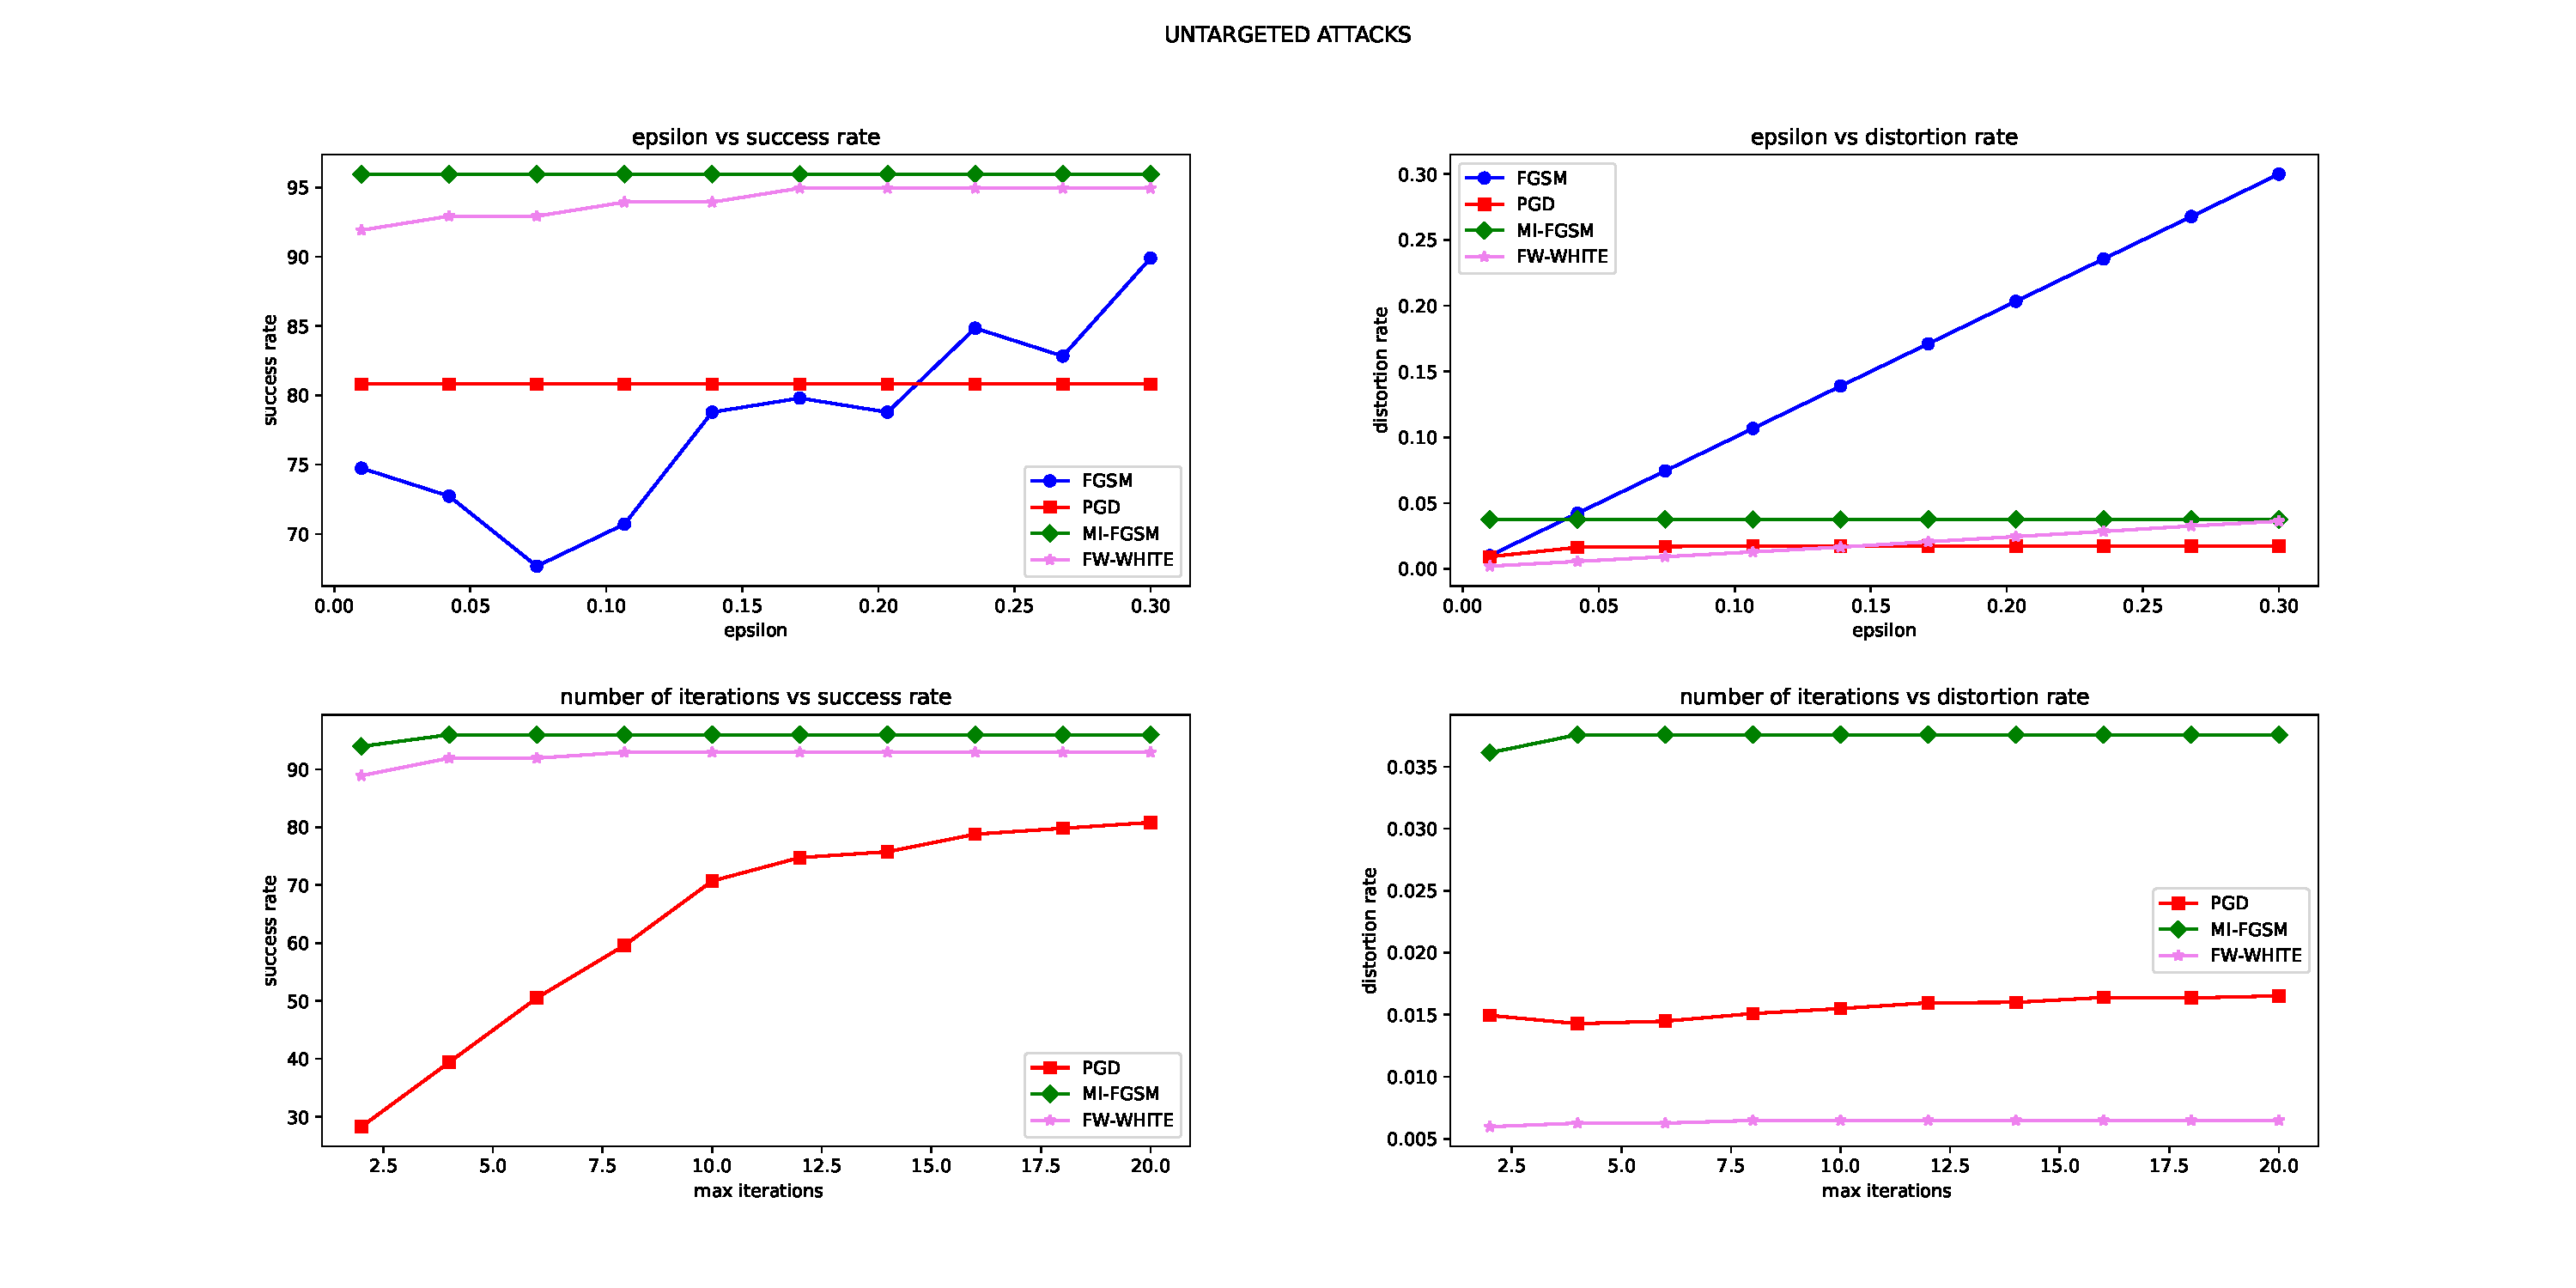
\includegraphics[width=\textwidth]{./Images/inceptionv3_untargeted_grid.pdf}\\
  \caption{InceptionV3 - untargeted attack } \label{incV3-unt}
\end{figure}

\begin{figure}[ht]
  \centering
  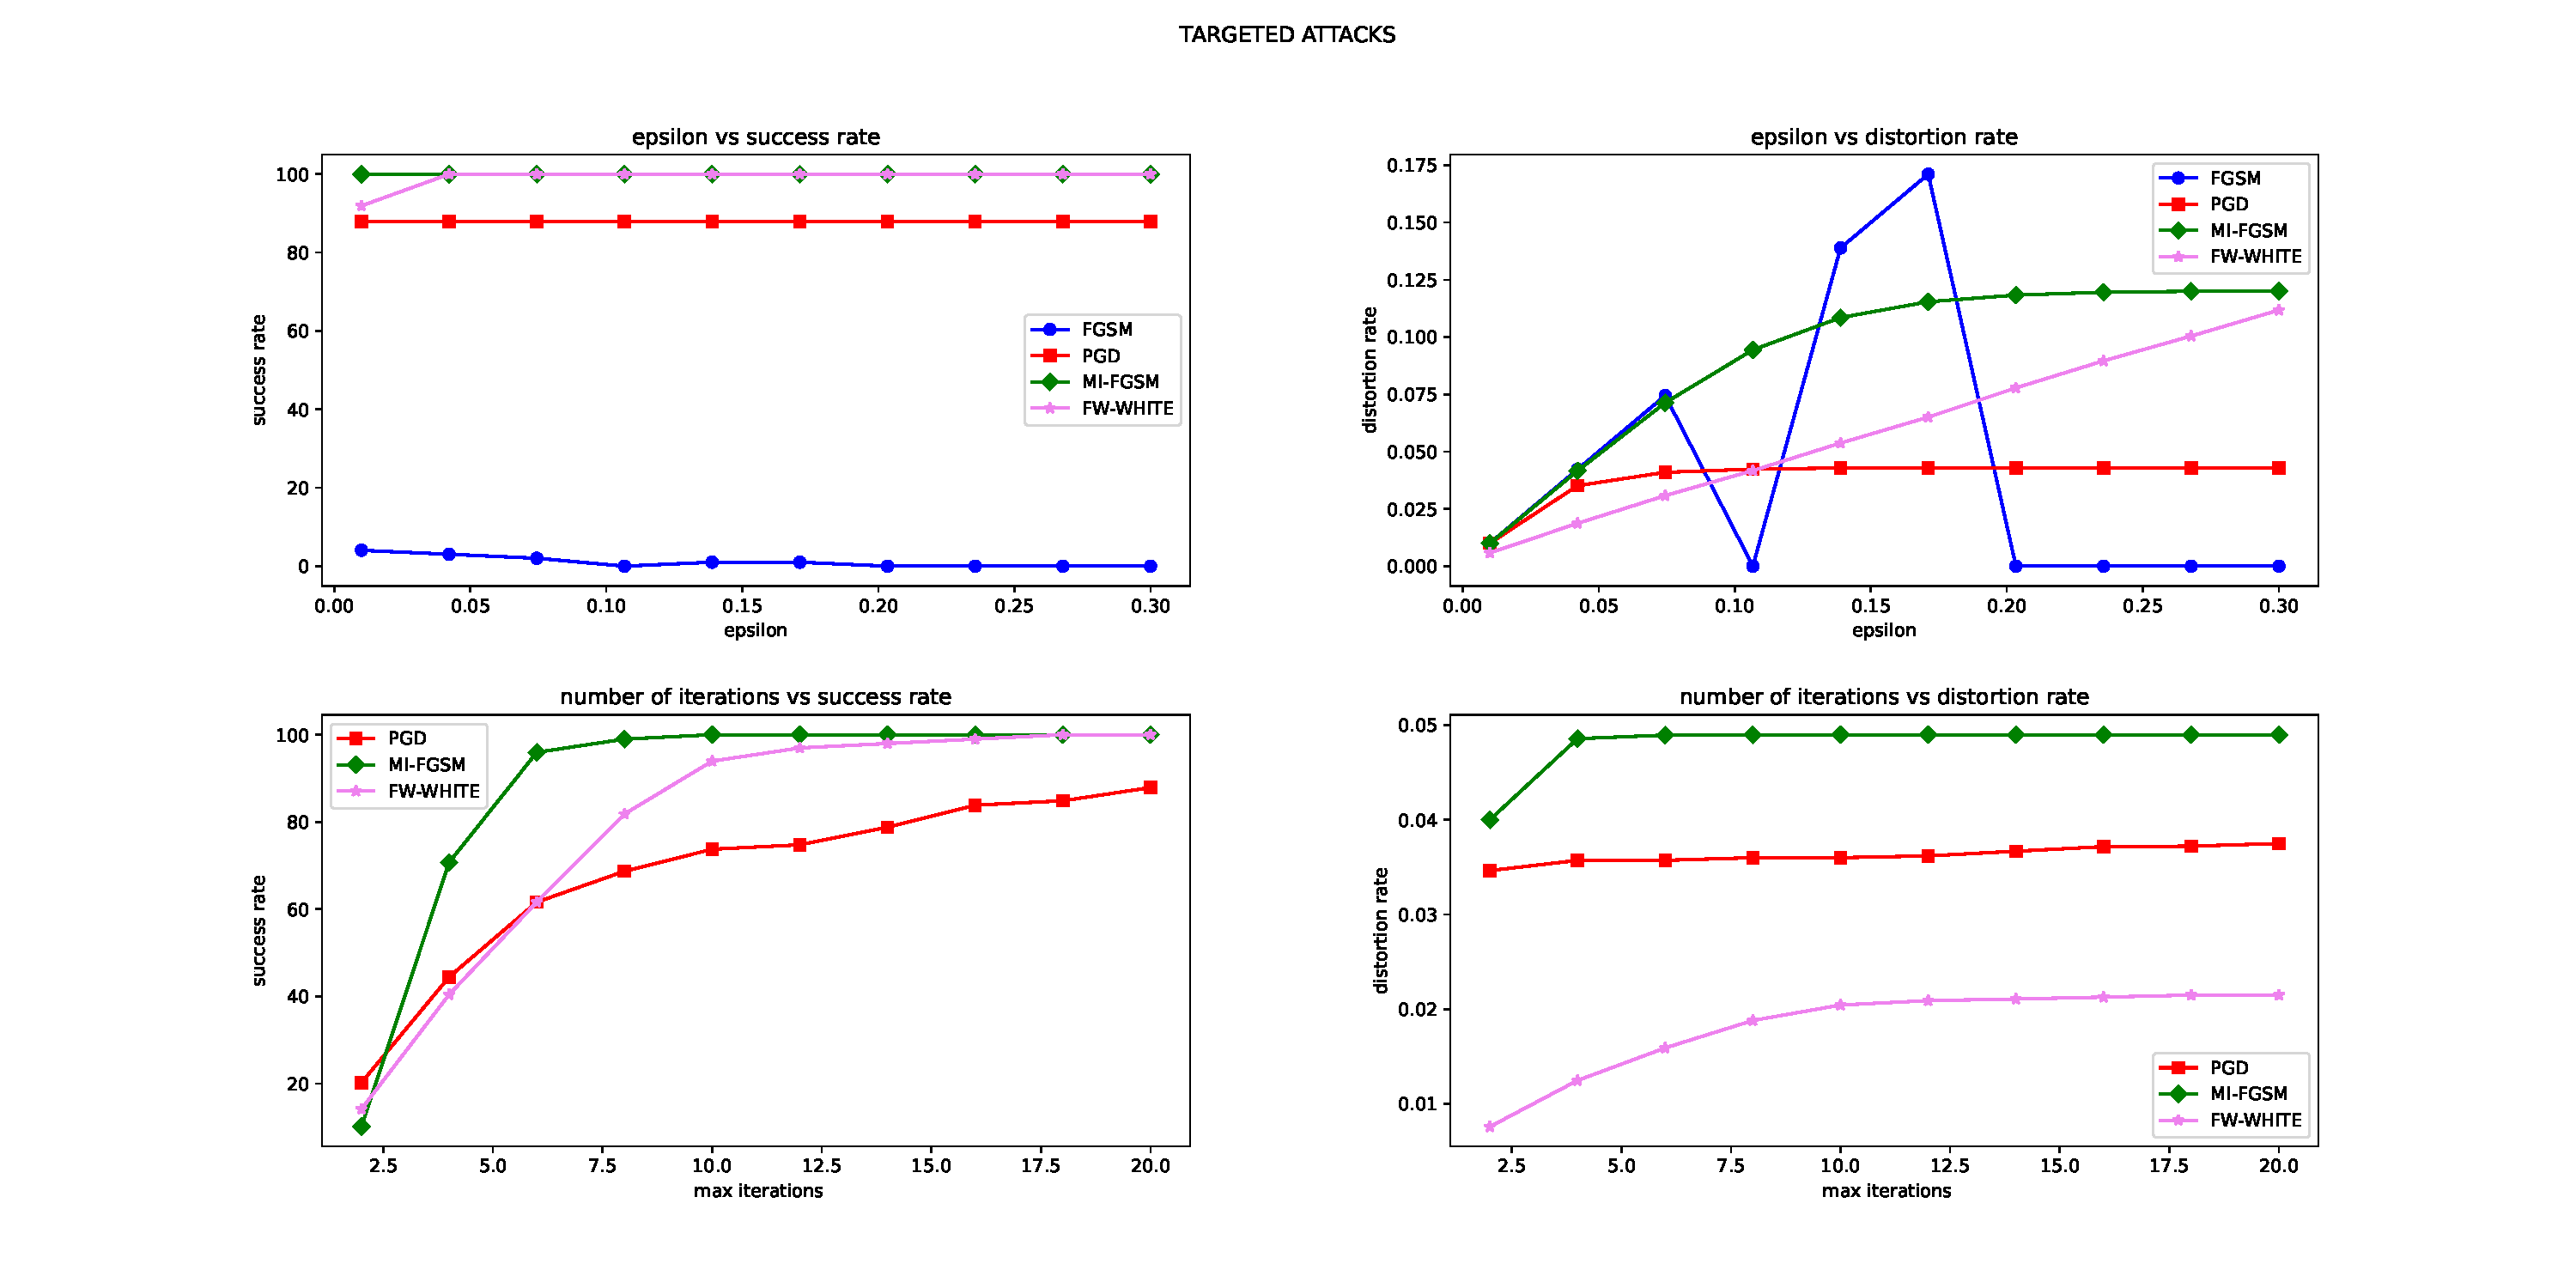
\includegraphics[width=\textwidth]{./Images/InceptionV3-targeted_grid.pdf}\\
  \caption{InceptionV3 - targeted attack } \label{incV3-t}
\end{figure}

\begin{figure}[ht]
  \centering
  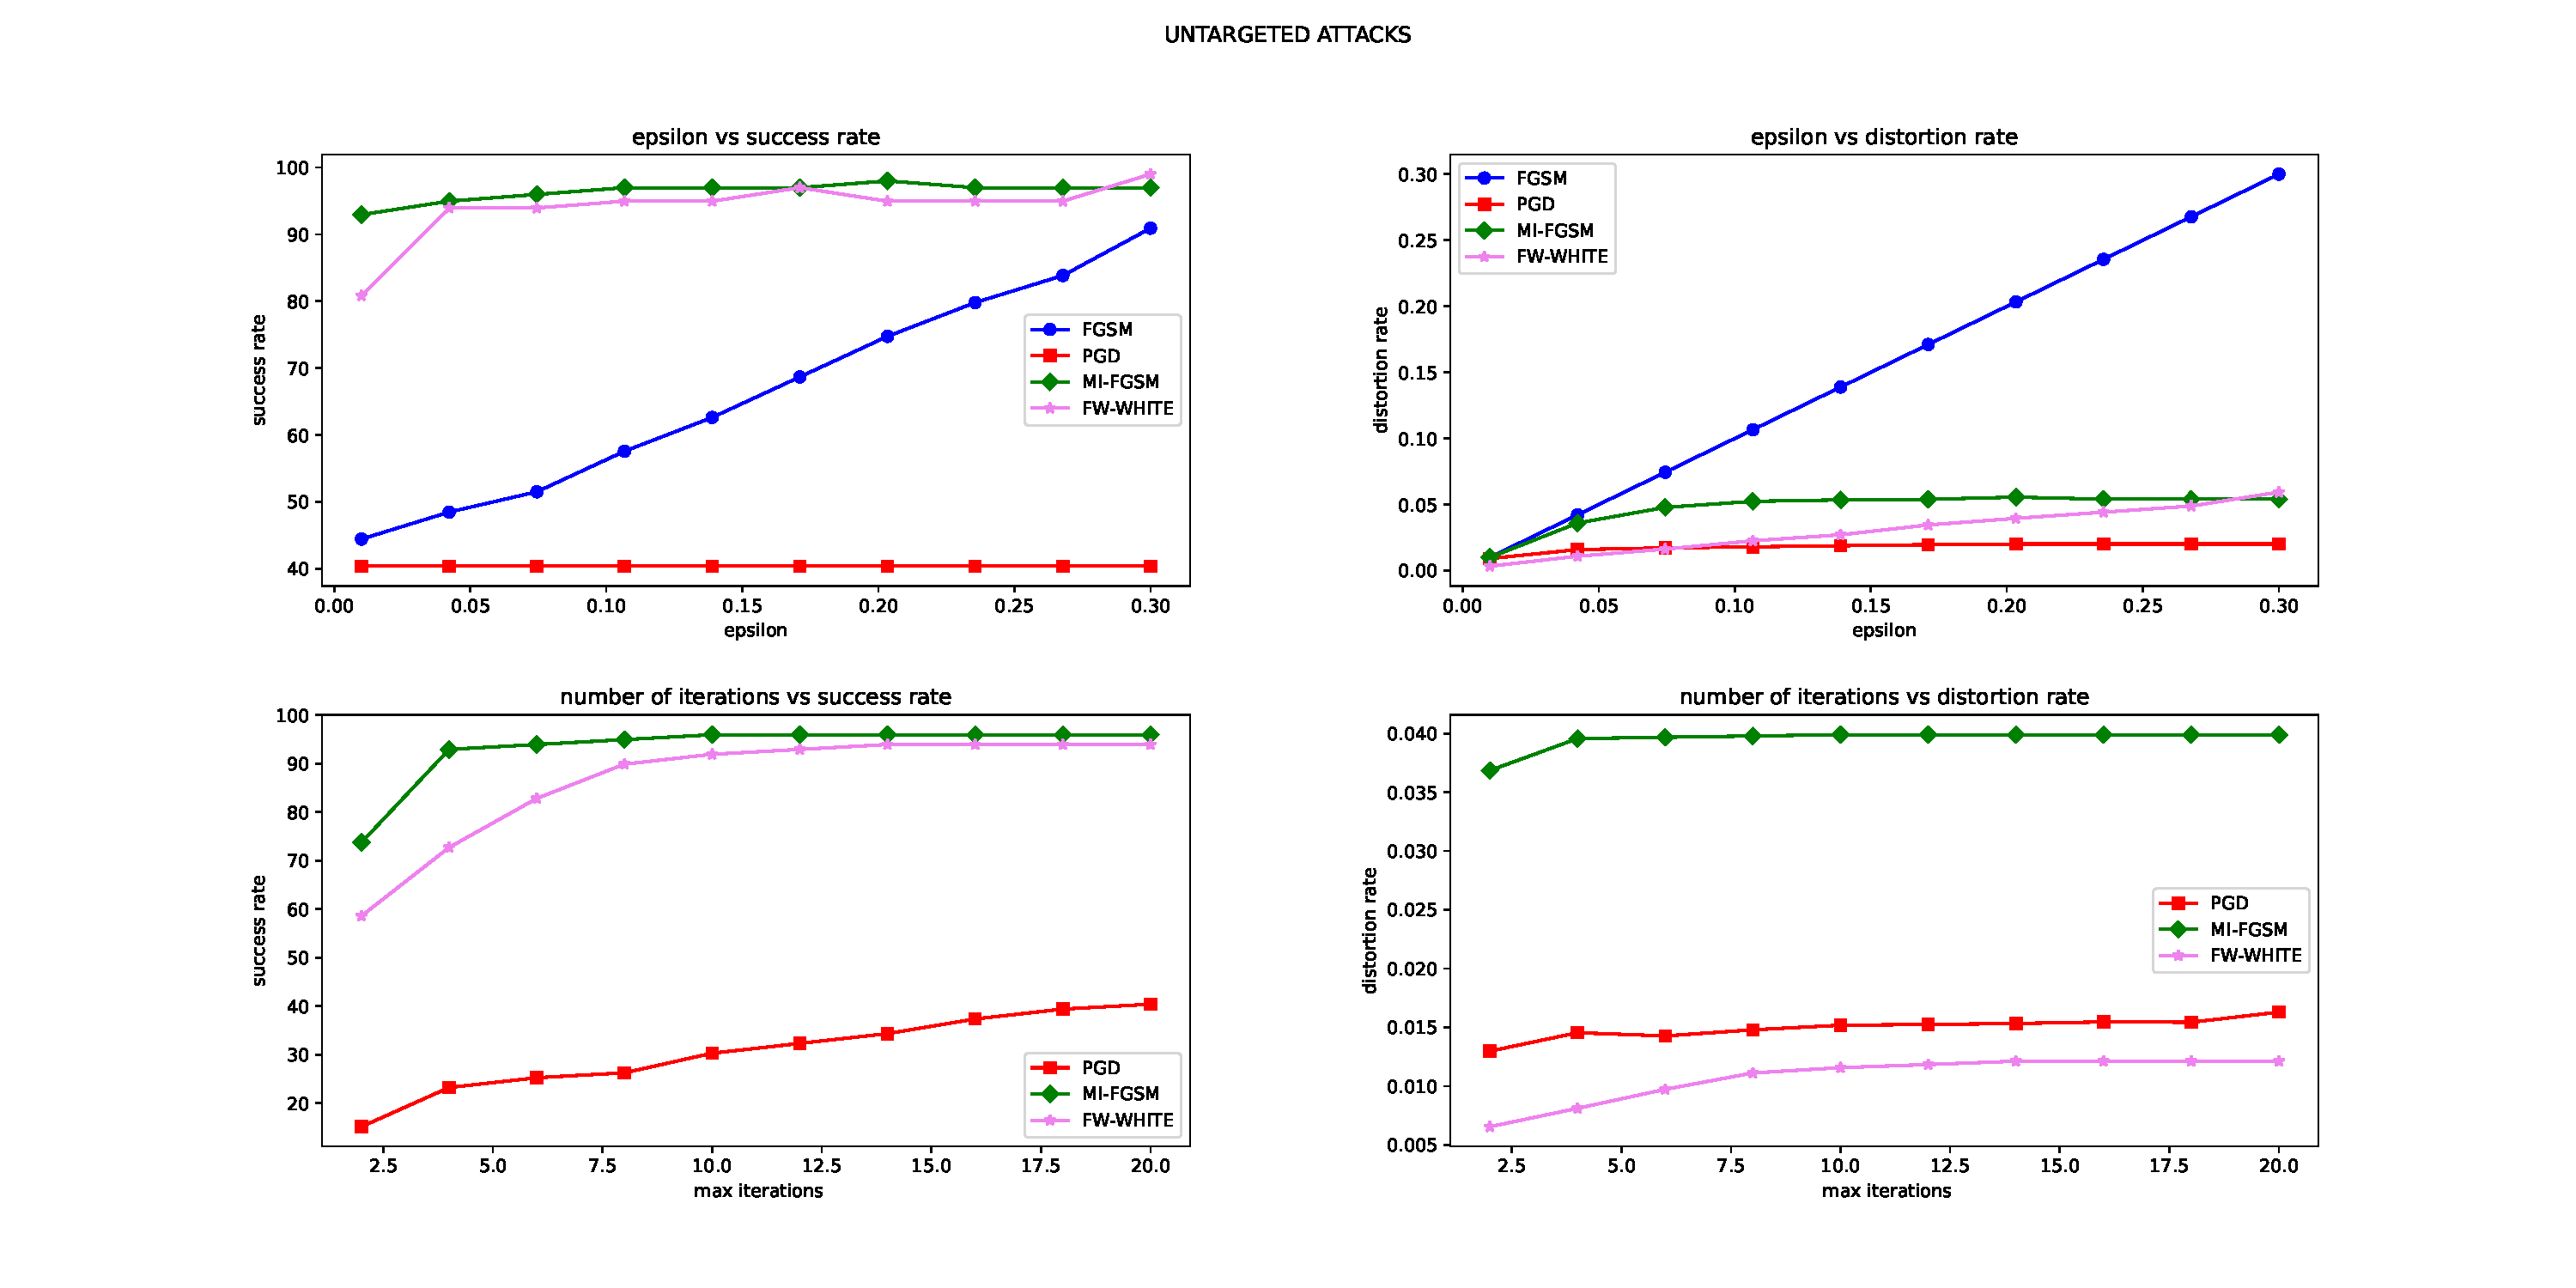
\includegraphics[width=\textwidth]{./Images/ResNet-untargeted_grid.pdf}\\
  \caption{ResNet - untargeted attack } \label{res-unt}
\end{figure}

\begin{figure}[ht]
  \centering
  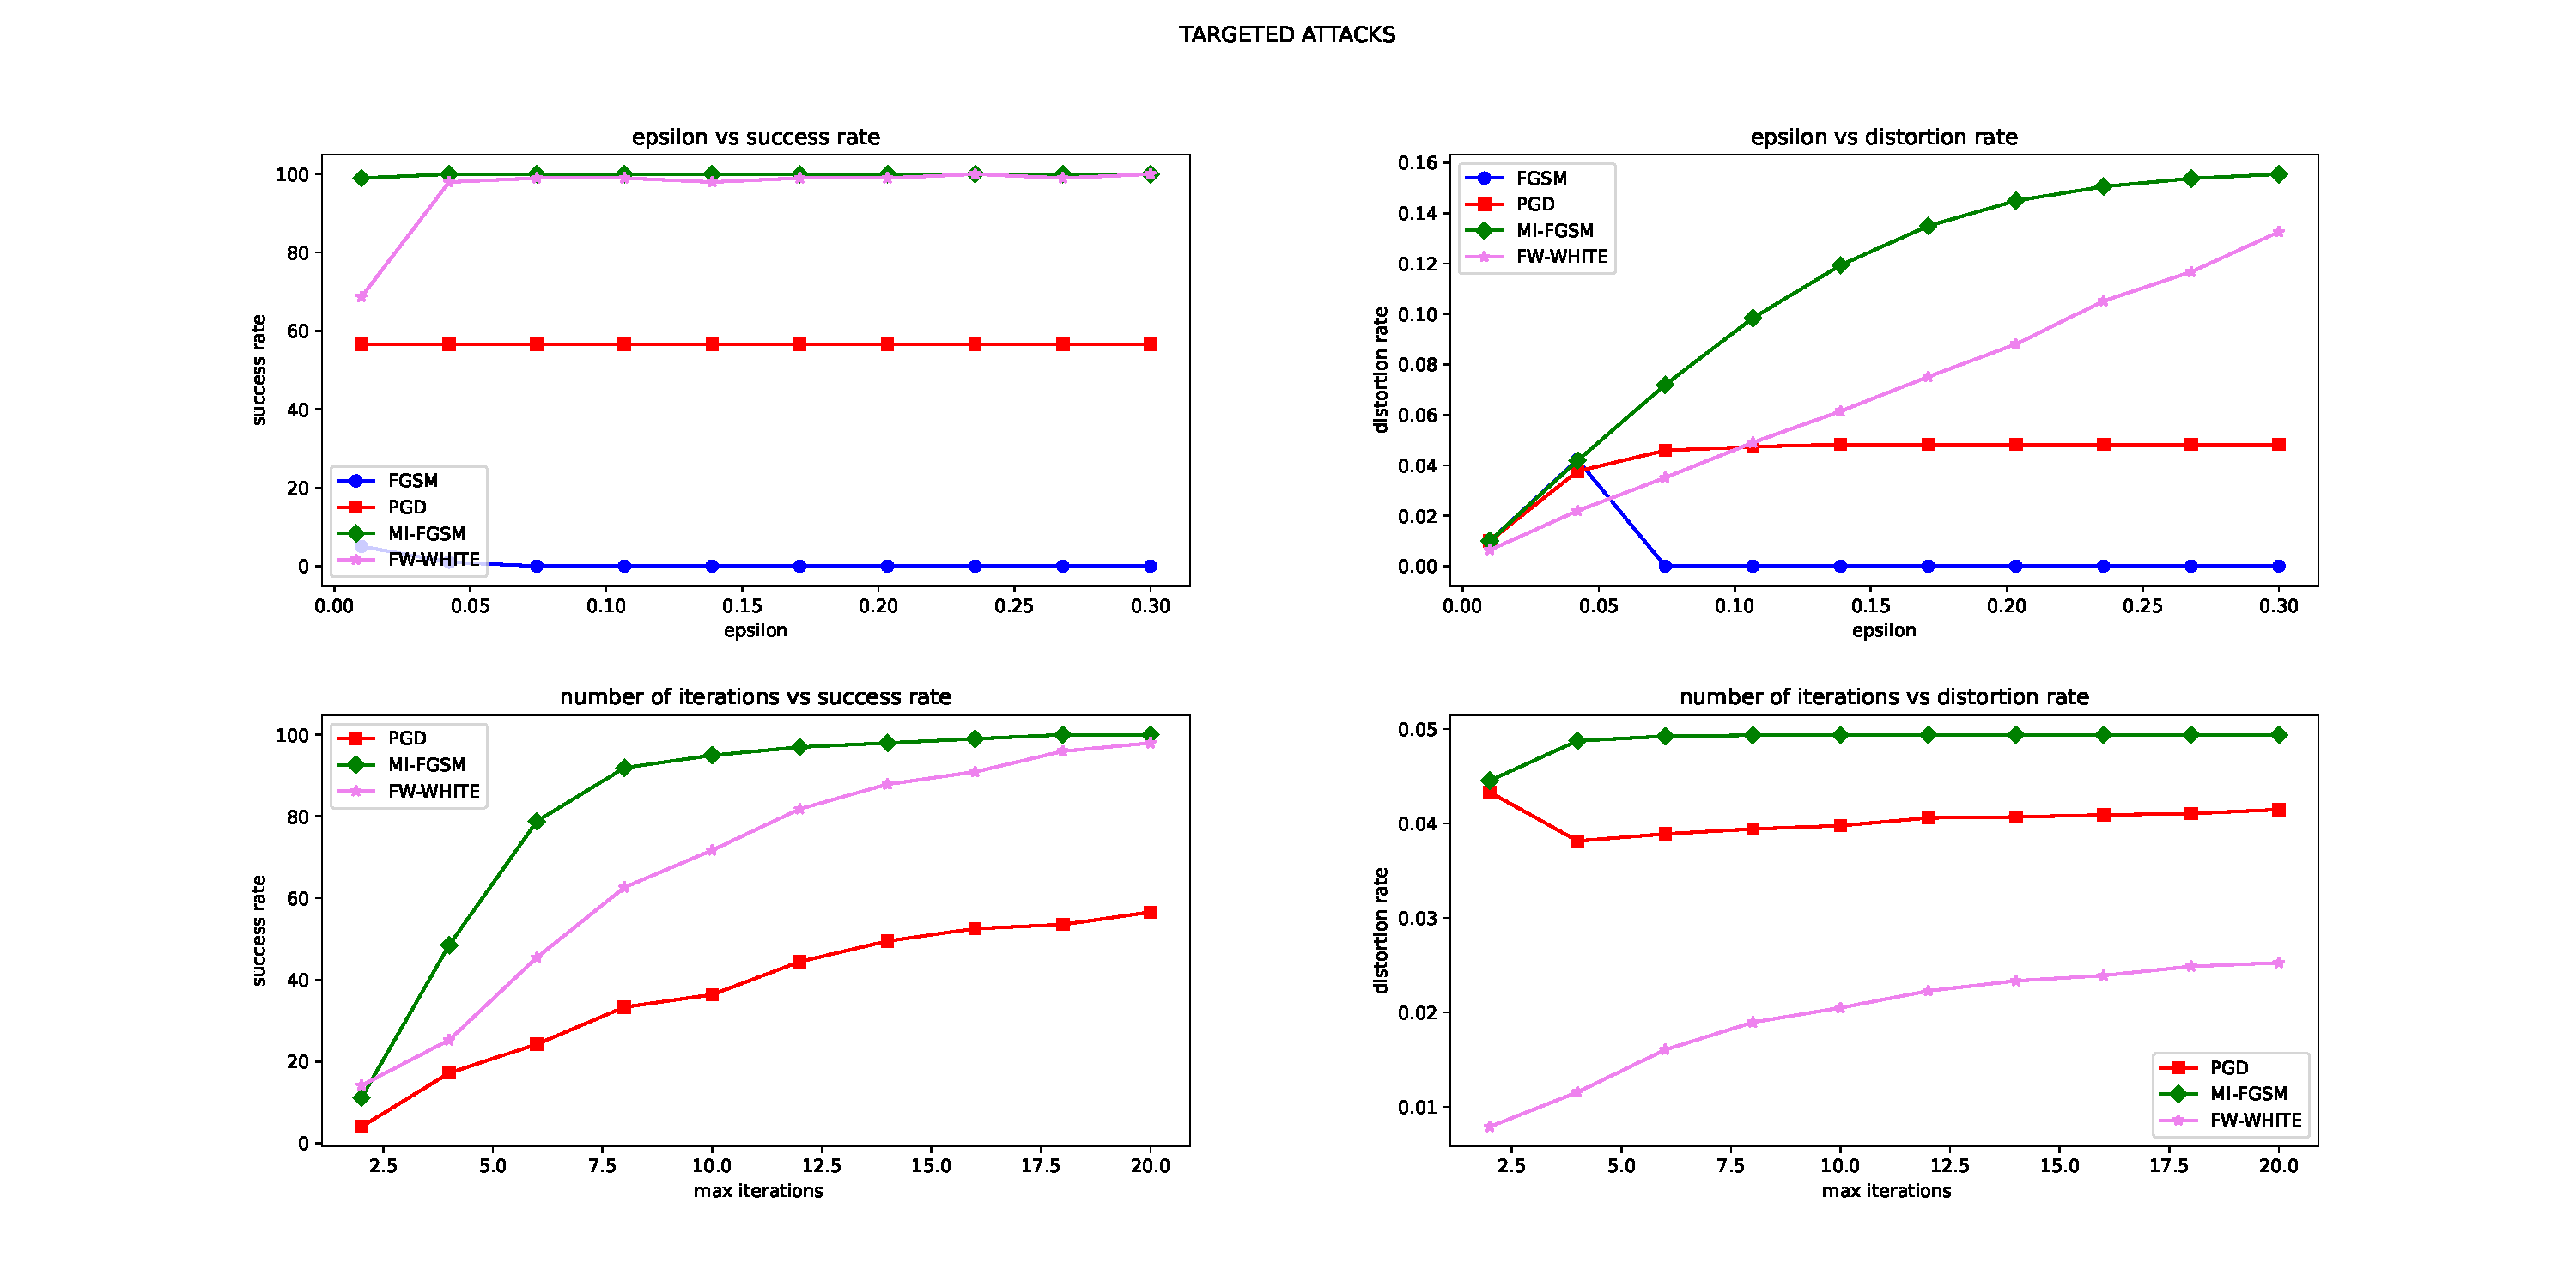
\includegraphics[width=\textwidth]{./Images/ResNet-targeted_grid.pdf}\\
  \caption{ResNet - targeted attack } \label{res-t}
\end{figure}

\begin{figure}[ht]
  \centering
  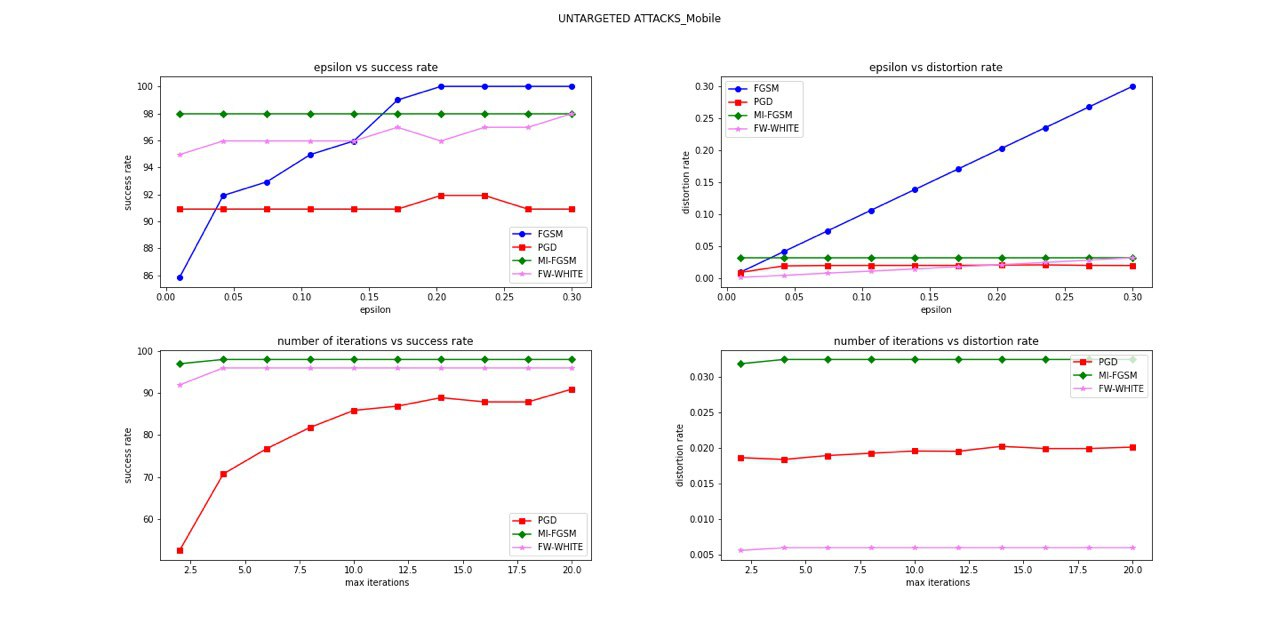
\includegraphics[width=\textwidth]{./Images/MobileNet-Untargeted.jpeg}\\
  \caption{MobileNet - untargeted attack } \label{mob-unt}
\end{figure}

\begin{figure}[ht]
  \centering
  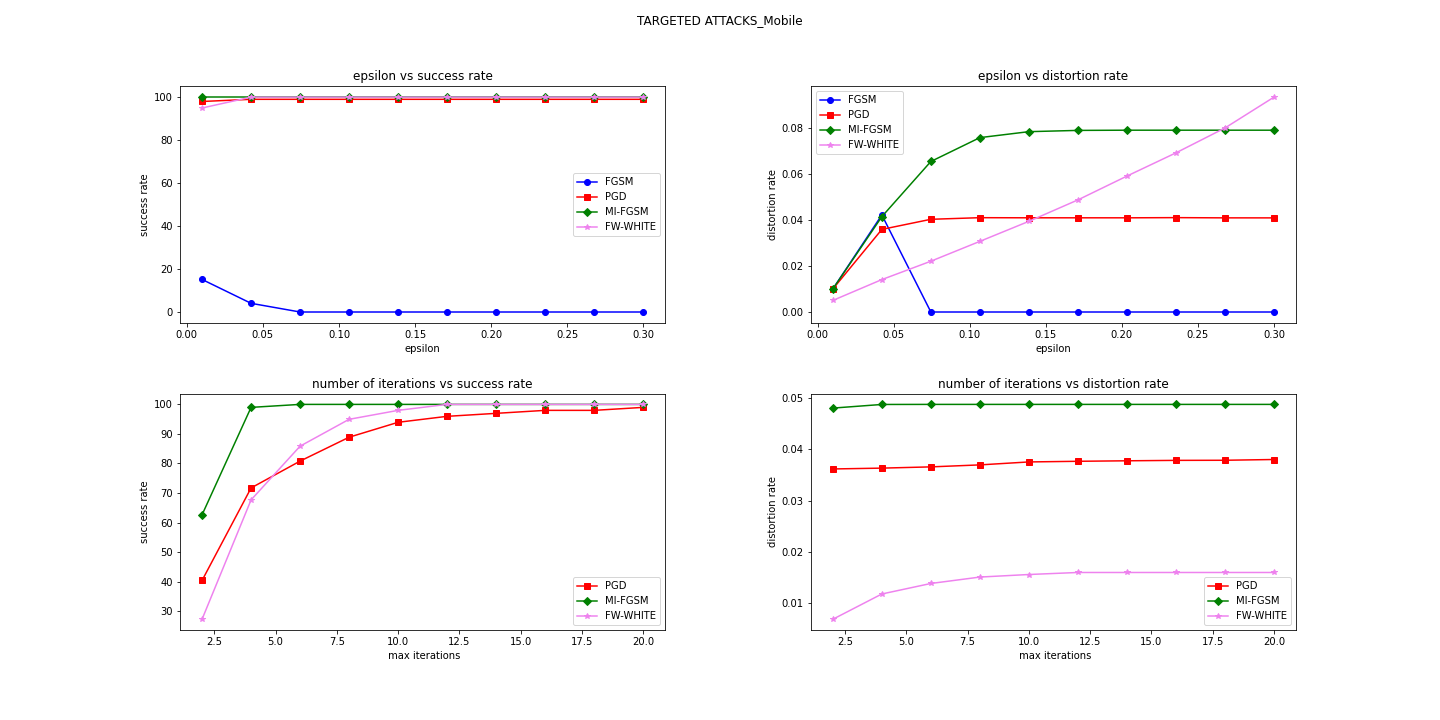
\includegraphics[width=\textwidth]{./Images/Mobile_Grid_Targeted.png}\\
  \caption{MobileNet - targeted attack } \label{mob-t}
\end{figure}




%-------------------------------------------------------------------------


\end{document}
